%Arquivo contendo o capítulo Metodologia
\chapter{Metodologia} \label{cap:metodologia}
A primeira etapa para o desenvolvimento do Pedal-to-Play será focada no levantamento de requisitos. Um dos requisitos já descrito nos objetivos deste trabalho é que este \textit{software} pretende ser multiplataforma e para garantir esta característica, pretende-se fazer uso das técnicas de desenvolvimento \textit{Web}. Segundo \citet{lopes2013}, o desenvolvimento \textit{Web} é democrático, aberto e acessível, pois praticamente, todo dispositivos \textit{mobile} possui um navegador (\textit{web browser}). Uma aplicação \textit{Web} garante acesso a um número maior de usuários do que uma aplicação nativa para um determinado dispositivo. Lopes também salienta que é cada vez mais comum usar as linguagens fundamentais da \textit{Web} para desenvolver aplicativos \textit{mobile}. \par

Demais requisitos envolverão: a definição dos \textit{frameworks} que serão utilizados; quais plataformas serão suportadas para execução da aplicação (sistemas operacionais \textit{mobile} e \textit{browsers}); a definição das ferramentas de desenvolvimento; as técnicas de gamificação a serem implementadas; as regras de negócio do sistema e os casos de uso. \par

Concluído o levantamento de requisitos, pretende-se iniciar a segunda etapa, a qual envolverá a prototipação da interface gráfica com o usuário (GUI\footnote{Acrônimo do inglês para \textit{Graphical User Interface}.}) e o desenvolvimento do \textit{template} do sistema. As interfaces terão como inspiração trabalhos e \textit{softwares} comerciais já existentes nessa categoria. O \textit{template} consistirá no desenvolvimento dos componentes comuns entre as telas da GUI, tais como a tela de \textit{login}, menu de navegação, cabeçalho, rodapé e tela de informações sobre o sistema. 

A terceira etapa do trabalho será focada na análise e modelagem do sistema. Envolverá o detalhamento dos casos de uso através de diagramas na linguagem UML (Unified Modeling Language\footnote{\url{http://www.uml.org/}}) para modelagem de sistemas. \par

A quarta etapa consistirá no desenvolvimento das funcionalidades do Pedal-to-Play e concomitantemente a dissertação da monografia e estudo das técnicas necessárias para implementação de cada funcionalidade. Pretende-se desenvolver as seguintes funcionalidades: \par

\begin{description}
\item[Rastreamento de Atividades] Envolve o uso dos recursos de \textit{hardware} dos dispositivo \textit{mobile} para captura de dados durante a prática da atividade de ciclismo. Pretende-se utilizar as funções do GPS\footnote{Acrônimo do inglês para \textit{Global Positioning System}.} para obter a distância do trajeto percorrido pelo usuário, possibilitando calcular a velocidade média e uma estimativa do total de calorias queimadas por ele.

\item[Módulo Avatar] Consiste nas funcionalidades do sistema responsáveis pela manutenção do avatar que representa virtualmente o usuário. Pretende-se desenvolver o avatar baseado em um conjunto de imagens bidimensionais, dividas em três categorias: o próprio avatar, os equipamentos dele e a bicicleta. Possibilitando ao usuário a customização de alguns atributos destas imagens (tais como cor e textura). A imagem \ref{fig:exavatar} é um exemplo ilustrativo da ideia do avatar a ser desenvolvido. 

\begin{figure}[h]
    \caption{Personagem da animação japonesa Yowamushi Pedal.}
    \centerline{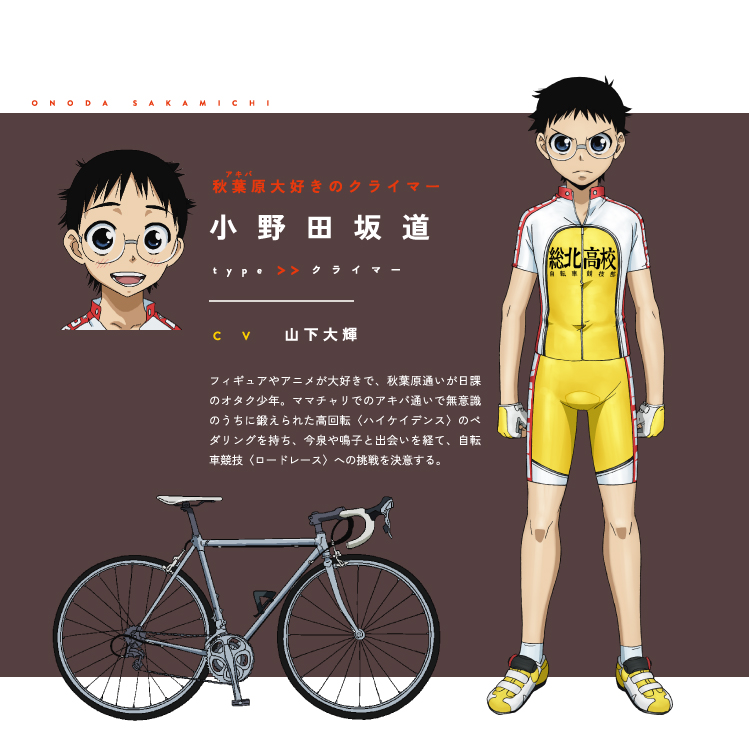
\includegraphics[width=20em]{figuras/exavatar.jpg}}
    \label{fig:exavatar}
\end{figure}
\centerline{Fonte: Página da \textit{Web} da qual a imagem foi retirada\footnote{Disponível em:  <\url{http://yowamushipedal.wikia.com/wiki/Onoda_Sakamichi}>. Acesso  em jul. 2015.}.}

\item[Lado do Servidor] O servidor consistirá na parte do sistema responsável pela persistência dos dados do usuário e a troca destes com a aplicação rodando no lado do cliente. \par

Atualmente o pódio das tecnologias para o desenvolvimento \textit{Web} do lado do Servidor está ocupado pelo PHP, em primeiro lugar; ASP.NET em segundo e o Java, em terceiro \cite{w3techs2015}. \par

Java \textit{Web} consiste na implementação das APIs de Servlets e JavaServer Pages (JSP). Servlet é a tecnologia usada pelo Java para geração de páginas HTML dinâmicas, são classes Java com HTML embutido. Páginas JSP consistem no inverso, são estruturadas como páginas HTML com código Java embutido. \par

ASP.NET é uma tecnologia da Microsoft, parte do .NET \textit{Framework} para desenvolvimento de aplicações \textit{Web}. As vantagens desta tecnologia envolvem a separação clara entre a interface do usuário e a lógica de programação; a familiaridade com o desenvolvimento \textit{desktop}; a ferramenta de desenvolvimento Visual Studio, com diversos recursos para facilitar o trabalho do desenvolvedor e a integração com todos os recursos do \textit{framework} .NET \cite{imar2014}. As desvantagens do ASP.NET são: sua limitação ao sistema operacional Windows e a licença de uso do Visual Studio não ser gratuita. \par

PHP é uma linguagem de programação presente em 10 milhões de sites no mundo inteiro. O PHP adiciona dinamismo às páginas estáticas e automatiza tarefas, diminuindo mão-de-obra. Possui portabilidade para várias plataformas \textit{desktop} (exemplos: Linux, Unix e Windows); possui código aberto e licença de uso gratuita; suporta vários bancos de dados (entre eles: MySQL, Oracle e PostgreSQL) \cite{niederauer2004, welling2003}. \par

Pretende-se usar a linguagem PHP para desenvolvimento do lado do servidor, pois comparado com as outras duas principais linguagens (ASP.NET e Java) o PHP se destaca por sua licença gratuita, portabilidade e suporte nativo (sem \textit{frameworks}) a funcionalidades que serão essenciais no software deste trabalho, tais como: gerenciamento de imagens, interpretação de arquivos JSON e acesso a banco de dados. \par

No quesito sistemas de gerenciamento de banco de dados (SGDB), os três mais usados atualmente segundo o \textit{site} da DB-Engines são o Oracle em primeiro lugar, o MySQL em segundo e o Microsoft SQL Server em terceiro. O MySQL possui licença de uso \textit{open source} e versão gratuita sem restrições, enquanto o Oracle e o Microsoft SQL Server são \textit{softwares} com licença de uso comercial, por estes motivos pretende-se fazer uso dele.

\item[Módulo Perfil do Usuário] Consiste no desenvolvimento da interface do perfil do usuário, contendo as principais informações dele, entre elas: nível, pontos, dados pessoais, avatar, \textit{ranking} e recompensas. Pretende-se que essa interface seja passível de customização.

\item[Módulo de Desafios] Envolve o mecanismo responsável pela geração de desafios, os quais consistem no cumprimento de certo objetivo proposto ao usuário. Pretende-se que os desafios sejam o meio para o usuário adquirir novos equipamentos, novas bicicletas, aumentar seu nível e \textit{ranking}, adquirir \textit{badges} e títulos.

\item[Integração com Redes Sociais] Envolve a implementação da funcionalidade que permite a integração com o Facebook, possibilitando ao usuário compartilhar seus dados, recompensas e aquisições nesta rede social. Esta funcionalidade é importante para divulgação do sistema e para propor engajamento social entre usuários do sistema e não usuários.
\end{description}

A etapa de conclusão deste trabalho será dedicada aos testes finais das funcionalidades desenvolvidas, à finalização da monografia e à defesa desta. \par 

Durante o decorrer deste trabalho serão estudados livros, trabalhos relacionados e tutoriais de uso das tecnologias necessárias para o  desenvolvimento do Pedal-to-Play. O material bibliográfico será pesquisado através de ferramentas de pesquisa eletrônica, como o Google Scholar e repositórios digitais, como o portal Lume, da Universidade Federal do Rio Grande do Sul. As palavras chave que direcionarão a pesquisa serão: \textit{mobile}, ciclismo, \textit{gamification}, \textit{web}, \textit{rastreamento de atividades} e geolocalização. Os tutorias serão buscados em plataformas de ensino digital, como o Mozilla Developer Network (MDN) e nos \textit{sites} oficiais de cada tecnologia. \par

Os produtos alvo deste trabalho serão o \textit{software} desenvolvido (gratuito e de código aberto) e a monografia, descrevendo o processo de pesquisa e desenvolvimento. \par
